\PassOptionsToPackage{svgnames}{xcolor}
\documentclass{book}
\usepackage[utf8]{inputenc}
\usepackage{graphicx}
\usepackage{listings}
\usepackage{hyperref}
\usepackage{amsmath}
\usepackage{xcolor}

\usepackage{tcolorbox}
\tcbuselibrary{skins,breakable}
\usetikzlibrary{shadings,shadows}

\newenvironment{myexampleblock}[1]{%
    \tcolorbox[beamer,%
    noparskip,breakable,
    colback=LightGreen,colframe=DarkGreen,%
    colbacklower=LimeGreen!75!LightGreen,%
    title={#1}, width=\textwidth]}%
    {\endtcolorbox}

\newenvironment{myalertblock}[1]{%
    \tcolorbox[beamer,%
    noparskip,breakable,
    colback=LightCoral,colframe=DarkRed,%
    colbacklower=Tomato!75!LightCoral,%
    title={#1}, width=\textwidth]}%
    {\endtcolorbox}

\newenvironment{myblock}[1]{%
    \tcolorbox[beamer,%
    noparskip,breakable,
    colback=LightBlue,colframe=DarkBlue,%
    colbacklower=DarkBlue!75!LightBlue,%
    title={#1}, width=\textwidth]}%
    {\endtcolorbox}

\newcommand{\code}[1]{\mbox{% added this percent
    \ttfamily
    \tcbox[
        on line,
        boxsep=0pt, left=4pt, right=4pt, top=2pt, bottom=1.5pt,
        toprule=0pt, rightrule=0pt, bottomrule=0pt, leftrule=0pt,
        oversize=0pt, enlarge left by=0pt, enlarge right by=0pt,
        colframe=white, colback=black!12,
        height=.8\baselineskip % added this (and guessed at .8)
    ]{#1}% added this percent
}}


\newtheorem{definition}{Definition}
\renewcommand{\chaptername}{Chapitre}

\begin{document}
\setlength{\parindent}{0cm}
\chapter{Git and GitHub}

Git et GitHub sont deux outils dont vous ne pourrez pas vous passer si vous voulez avoir une carrière qui inclut de la programmation. Normalement, vous devriez tous avoir un compte GitHub et avoir déjà installé Git sur votre ordinateur. Ces outils sont utilisés dans les cours d'introduction à la programmation puisqu'ils sont essentiels. Vous connaissez probablement plusieurs informations qui se trouvent dans ce tutoriel. Toutefois, il est possible que vous ne les compreniez pas suffisament pour vous en servir correctement au quotidien. Le but de ce tutoriel est de faire un rappel et de vous apprendre la base de Git et GitHub qui n'a pas été enseignée durant le cours d'introduction à la programmation. \\

Git est un outil de versionnage et d'hébergement de code. Git permet d'héberger son code sur un serveur, ce qui a l'avantage d'éviter d'avoir une seule version locale sur votre ordinateur et de faciliter la collaboration. En hébergeant votre code dans un dépôt central, vous pouvez l'utiliser et le modifier à partir de différents ordinateurs, tout en étant sûr que vous avez toujours une sauvegarde. Puisque le code est hébergé sur un serveur, plusieurs développeurs peuvent développer chacun de leur côté sur leur ordinateur, puis fusionner le code à la version globale, qui pourra ensuite être utilisée par tous les autres collaborateurs. Il est recommandé d'utiliser Git même lorsque vous travaillez seul, pour avoir accès aux différentes versions du projet si vous faites une erreur ou si votre ordinateur a des problèmes. \\

Chacun de vos projets sera placé dans un dépôt\footnote{Tout au long de ce tutoriel, j'utiliserai dépôt au lieu de \emph{repository}.}. Dans votre ordinateur, le dépôt local sera simplement un dossier qui contient l'entièreté de votre code. Toutefois, il sera aussi synchronisé sur un dépôt central. Le dépôt central est la version hébergée sur les serveurs de GitHub. Dans les prochaines sections, je vous montrerai à utiliser les différentes lignes de commande Git. 

GitHub est un serveur qui utilise Git comme interface avec l'utilisateur. C'est GitHub qui va héberger le code. Pour déposer votre code sur GitHub, vous devrez utiliser Git. GitHub est utile entre autres pour le partage de code. En effet, il est possible d'accéder au code d'un collègue simplement grâce à un url. Il existe de plus beaucoup de dépôts publics, que vous pourrez utiliser pour vos différents projets. Ils proposent de plus plusieurs outils qui permettent de faciliter le développement logiciel. 

Avant de commencer à présenter les commandes git, au cas où vous n'auriez toujours pas installé Git sur votre ordinateur, je vous fournis les étapes. 

\section{Configuration de Git}

Comme mentionné dans l'introduction, vous devriez déjà avoir un compte gitHub, avoir téléchargé Git et l'avoir configuré. Toutefois, si jamais ce n'est pas fait, voici comment le faire. 

Commencez par ouvrir votre terminal et taper "git". La sortie de votre terminal\footnote{Quand je parle de Terminal, vous pouvez utiliser le terminal, git bash, etc. Tout ce qui compte, c'est que vous soyez en mesure d'utiliser des lignes de commande.} devrait ressembler à celle de la figure~\ref{fig:check_if_git}. Si c'est le cas, alors Git est déjà installé et vous pouvez passer à la prochaine section. 

\begin{figure}[!h]
    \centering
    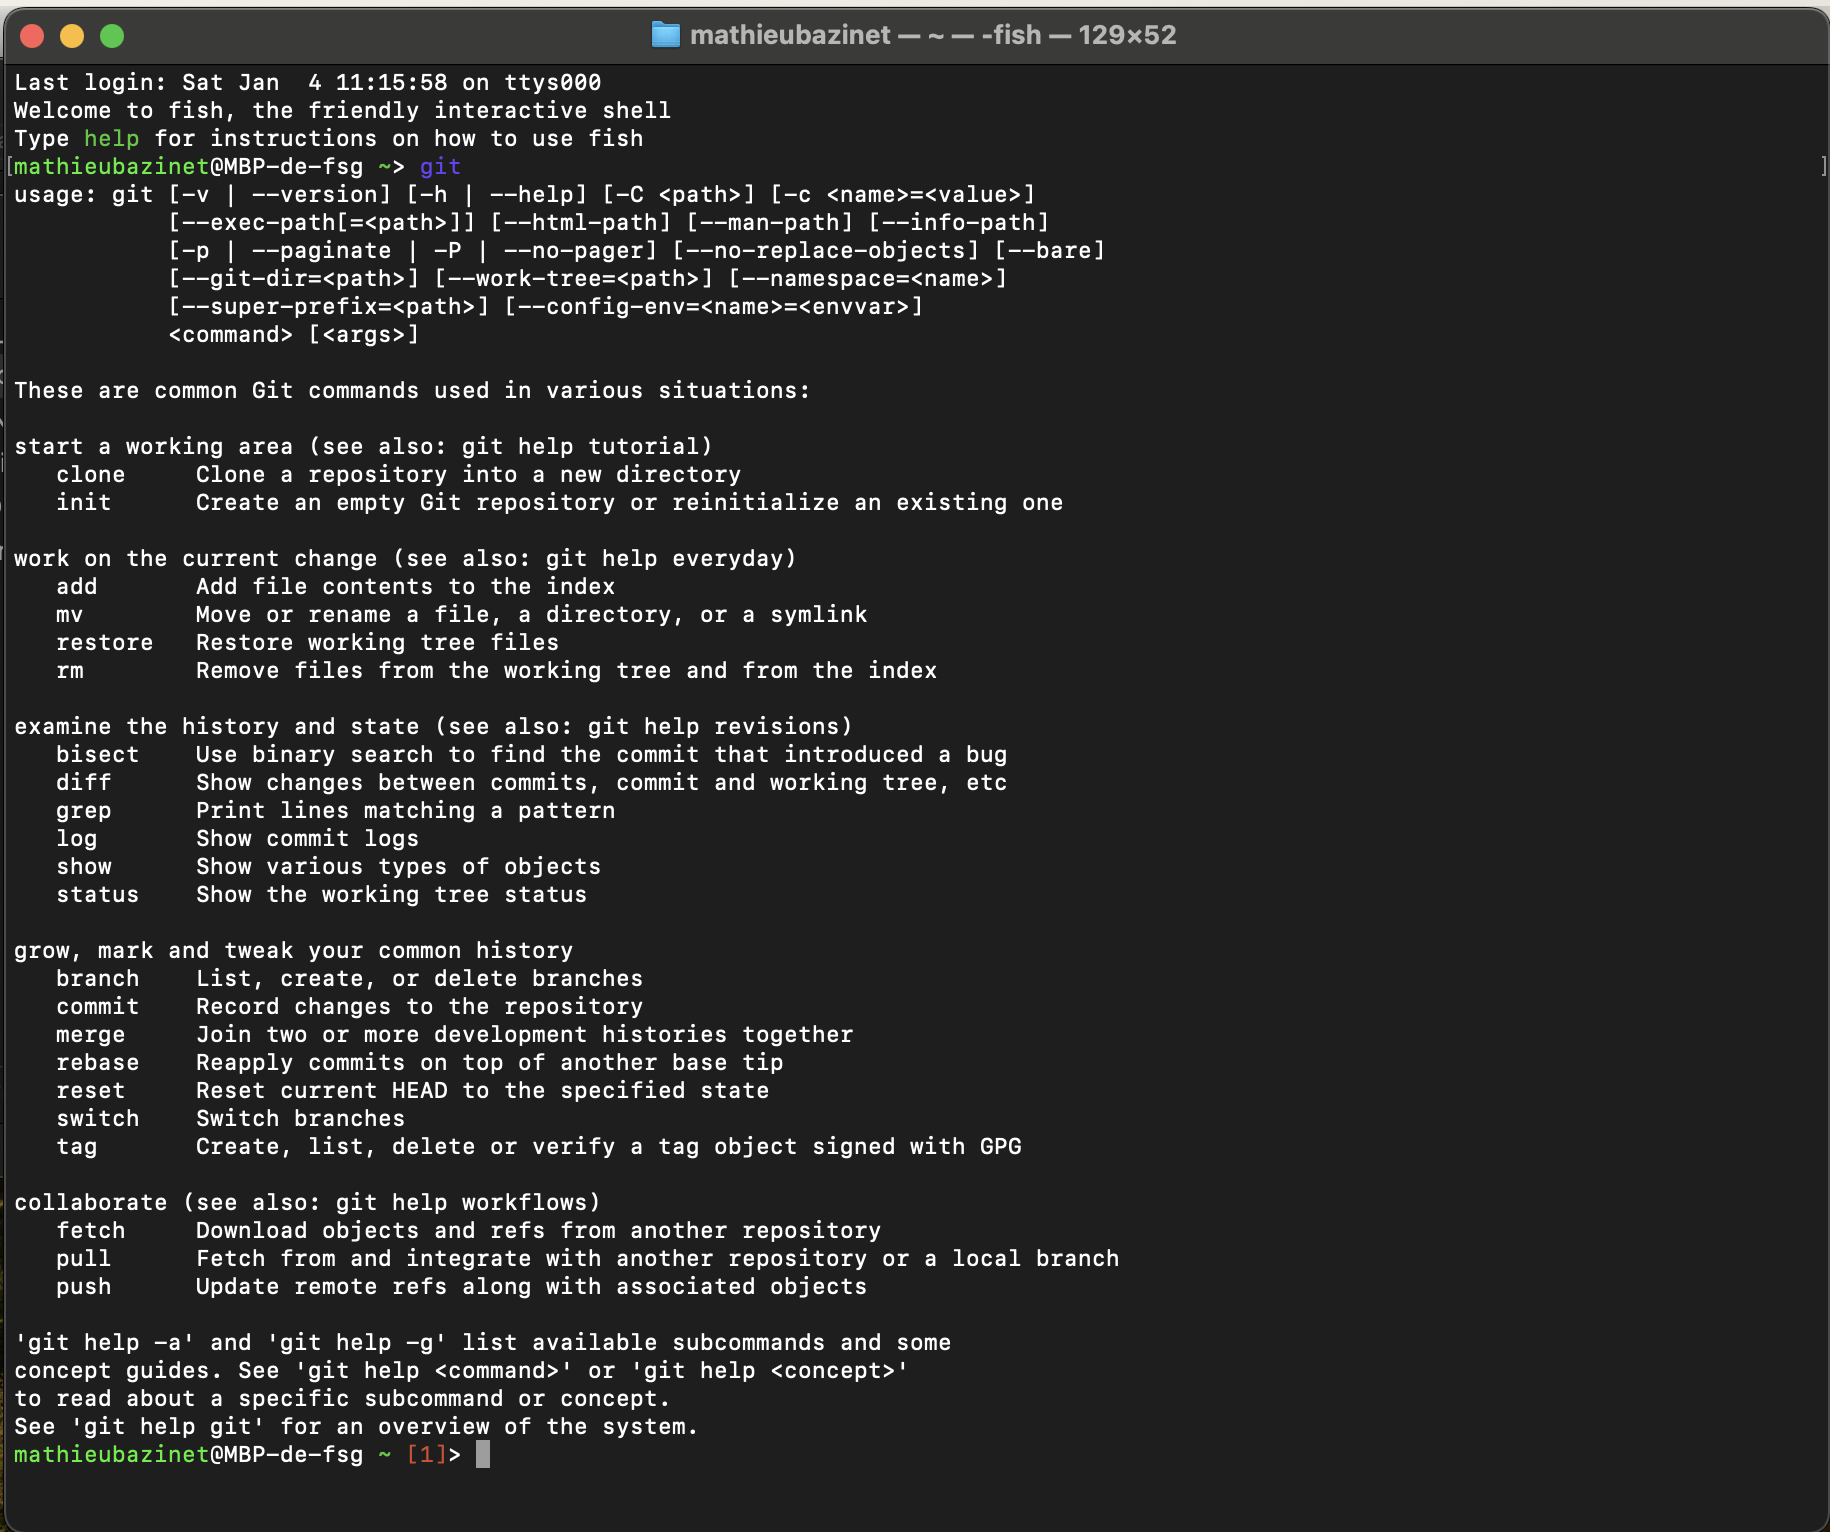
\includegraphics[width=0.8\textwidth]{images/check_if_git.png}
    \caption{Sortie attendue dans le terminal lorsque la commande ``git'' est tapée dans le terminal.} \label{fig:check_if_git}
\end{figure}

Si Git n'est pas installé, vous devrez le télécharger. Normalement, sur Linux, il devrait déjà être installé. Sur Windows, téléchargez le \href{https://git-scm.com/}{ici}. Pour les utilisateurs de Mac, nous recommandons de le télécharger en installant Xcode. Dans le terminal, tapez la commande suivante \code{xcode-select --install}.

Maintenant, vous devez configurer Git pour qu'il ait accès à votre profil GitHub. Dans le terminal, veuillez recopier les commandes suivantes puis remplacer votre email ainsi que votre nom d'utilisateur GitHub. 

\code{git config --global user.email "<votre-adresse-email>"} \\
\code{git config --global user.name "<votre-nom-d'utilisateur-github>"} \\
	
Pour les utilisateurs d'un Mac, vous ne pourrez pas utiliser un mot de passe pour vous connecter à GitHub à travers Git. Vous devrez vous créer un \emph{personal access token}, en suivant les instructions \href{https://docs.github.com/fr/authentication/keeping-your-account-and-data-secure/managing-your-personal-access-tokens\#cr%C3%A9ation-dun-personal-access-token-classic}{ici}. À chaque fois que Git vous demandera un mot de passe, vous \textbf{devez} utiliser le token de GitHub.


\section{Première étape avec Git et GitHub}

Comme première étape, vous allez clôner le dépôt de ce tutoriel. Vous aurez ainsi accès à ce fichier PDF, qui pourra vous être utile plus tard. Lors du clônage d'un dépôt, Git va créer une copie locale du dépôt sur votre ordinateur, que vous pourrez modifier ensuite. 

Pour clôner le dépôt, il vous est nécessaire d'avoir son url. Pour ce faire, suivez les étapes de l'exercice suivant.
\begin{myexampleblock}{Exercice : Trouver le dépôt du tutoriel}
    \begin{enumerate}
        \item Sur GitHub, cherchez ``Club d'intelligence artificielle de l'Université Laval''.
        \item Par défaut, GitHub cherche dans les noms de dépôt. Sélectionnez ``Users'' dans la barre de gauche.
        \item Sélectionnez ``Club d'intelligence artificielle de l'Université Laval''
        \item Cherchez maintenant le dépôt nommé ``tutoriels-h2024'' et cliquez dessus.
    \end{enumerate}
\end{myexampleblock}

Prenez le temps d'observer le contenu du dépôt. Vous y trouverez les dossiers associés aux trois tutoriels de la session, ainsi que quatre fichiers : \code{.gitignore}, \code{LICENSE}, \code{README.md} et \code{requirements.txt}. Un bon dépôt devrait toujours contenir ces quatres fichiers. Nous y reviendrons plus tard, après avoir clôné le dépôt. \\

Nous voulons maintenant clôner le dépôt. Pour ce faire, nous utiliserons notre première commande Git.

\begin{myblock}{\href{https://git-scm.com/docs/git-clone}{git clone}}
    La commande \texttt{git clone <url-du-repo>} permet de créer une copie locale du projet. 
\end{myblock}

\begin{myexampleblock}{Exercice : Clôner le dépôt du tutoriel}
    \begin{enumerate}
        \item Cliquez sur le bouton vert marqué ``Code'' et sélectionnez ``HTTPS''.
        \item Copiez le lien.
        \item Dans le terminal, tapez \code{\texttt{git clone <lien-du-repo>}}.
    \end{enumerate}
\end{myexampleblock}

Maintenant que vous avez téléchargez le dépôt, ouvrez un par un les fichiers. Je vous présenterai maintenant les quatre fichiers essentiels à un bon dépôt GitHub.

\subsection{README}

Le README est le premier contact entre l'utilisateur et le dépôt. C'est un fichier markdown qui doit donner les informations nécessaires à utiliser le code du dépôt. Le README va contenir un titre ainsi qu'une description du projet. Ainsi, on doit savoir quel est le but du projet ainsi que comment l'utiliser. Plus la description est claire, plus il est probable que d'autres utilisateurs veuillent utiliser votre code. Il est donc important de faire un beau README. \\

Par exemple, si c'est un dépôt qui fournit une fonction ou un groupe de fonction, donnez un exemple simple d'utilisation. Par exemple, si mon projet fourni la fonction \code{\texttt{reverse\_name}} suivante\footnote{Exemple généré par ChatGPT sous ma demande.}

\begin{lstlisting}[language=Python]
def reverse_name(name):
    return name[::-1]
\end{lstlisting}

alors je pourrais fournir l'exemple suivant :
\begin{lstlisting}[language=Python, commentstyle=\small\ttfamily,]
# Input your name
my_name = "John Doe"

# Reverse your name using the function
reversed_name = reverse_name(my_name)

# Print the reversed name
# This will output "Reversed Name: eoD nhoJ"
print("Reversed Name:", reversed_name)
\end{lstlisting}

Pour la majorité des projets de programmation, vous devriez spécifier la version de Python que vous avez utilisés lors du développement, ainsi que fournir un fichier \code{requirements.txt}. De plus, si vous avez utilisés le code d'une autre personne, vous devez indiquer d'où provient ce code.

Pour plus d'information, je vous recommande ce \href{https://www.freecodecamp.org/news/how-to-write-a-good-readme-file/}{blog}.
\subsection{LICENSE}

\textcolor{red}{Disclaimer : Je ne suis pas un expert légal, donc il ne faut pas croire tout ce que je dis.\\}

La licence n'est pas un document que vous allez consulter souvent. Le but de la licence est de savoir ce que pouvez faire et ce que vous ne pouvez pas faire avec le code dans le dépôt. Les licences les plus classiques sont CC-BY 4.0, MIT, GNU et Apache 2.0. Généralement, vous devriez pouvoir utiliser et modifier le code sans problème, tant que vous citez le matériel emprunté. Il faut toutefois faire attention si jamais vous faites un projet de recherche ou un produit dans une compagnie, car certaines licences nécessitent que tout code qui utilise le projet soit sous la même licence et potentiellement rendu public. \\

S'il n'y a pas de licence, c'est équivalent à "ne pas toucher". Il y a beaucoup de chercheurs qui ne mettent pas de licence en se disant que ça devient "open-source" et peut-être utilisé par n'importe qui, mais c'est le contraire. Pas de licence veut dire que tous les droits sont à l'auteurs et que tu ne peux pas utiliser le code. Dans un petit projet, ce n'est pas très grave, personne ne va vous taper sur les doigts. Si vous faites de la recherche ou vous voulez publier du code et laisser la communauté l'utiliser, il faut demander la permission aux auteurs ou suivre la licence\footnote{Je vous encourage à aller lire cette page web : \url{https://choosealicense.com/no-permission/}}. \\

Lorsque vous créez un dépôt, je vous encourage à suivre \href{https://docs.github.com/fr/repositories/managing-your-repositorys-settings-and-features/customizing-your-repository/licensing-a-repository}{la procédure de GitHub} pour la sélection de licence. Si vous avez d'autres questions, je vous recommande le site \href{https://choosealicense.com/}{Choose A License}.

\subsection{.gitignore}
Le fichier .gitignore n'est pas le fichier le plus intéressant. C'est purement un fichier utilitaire. Il va être utile uniquement si l'utilisation de votre code crée des fichiers qui ne doivent pas se retrouver sur GitHub. Par exemple, si votre code télécharge MNIST, on ne veut pas qu'il se retrouve sur GitHub. Un autre exemple, directement dans le dossier Tuto1-GitHub, vous trouverez un fichier ``.tex''. Si vous compilez le fichier, vous aurez un pdf ainsi que des fichiers avec des extensions tels que ".aux", ".fls", ".log", ".out", etc. Ces fichiers ne sont pas pertinents et je ne veux pas oublier de les enlever et mettre des fichiers inutiles sur GitHub. Si vous regardez le fichier .gitignore, vous verrez en bas les lignes suivantes : 

\begin{lstlisting}
*.aux
*.fdb_latexmk
*.fls
*.out
*.synctex.gz
\end{lstlisting}

Vous ne les trouverez pas sur GitHub, puisqu'ils sont automatiquement ignorés. L'astérisque au début veut dire : tous les fichiers de style \code{<nom\_du\_fichier>.aux} va être matché par *.aux. \\

Pour plus d'information, je recommande la \href{https://git-scm.com/docs/gitignore}{documentation de Git}.


\subsection{requirements.txt}
En plus de la version de Python donnée dans le README, il est de bonne usage de donner la version des librairies utilisées par le projet. Vous garantissez que le code va fonctionner et sera reproductible si l'utilisateur utilise la version des librairies que vous avez utilisés. Pour produire le fichier, vous pouvez utiliser la commande suivante :

\code{\texttt{pip freeze $>$ requirements.txt}}\\

Quand vous ouvrez un dépôt qui contient un fichier \code{requirements.txt}, vous pouvez installer toutes les dépendances en utilisant la commande suivante :

\code{\texttt{pip install -r requirements.txt}}


\section{Créer un dépôt Git}\label{sec:creer_depot}

Vous allez maintenant créer un dépôt Git. Techniquement, il est possible de créer un dépôt avec \texttt{git init}. Je trouve qu'il est beaucoup plus facile de le faire directement sur GitHub. Vous devrez : 

\begin{itemize}
    \item Choisir un nom pour le dépôt
    \item Ajouter une description courte
    \item Choisir si le dépôt est privé ou public
    \item Ajouter un README
    \item Ajouter un .gitignore
    \item Choisir une licence
\end{itemize}

Lorsque vous choisissez un nom pour votre dépôt, il est important de savoir qu'il existe (au moins) deux noms de dépôts qui sont réservés pour des usages spécifiques. En effet, si vous choisissez votre nom d'utilisateur, GitHub va rajouter un README sur votre page d'accueil. Si vous choisissez un repo de style \code{<nom-d'utilisateur>.github.io}, GitHub va vous permettre d'héberger un site web. \\

En effet, commencez par aller voir le profil GitHub de \href{https://github.com/NathanielDamours}{Nathaniel D'Amours}. Vous aurez généralement accès aux dépôts publics de Nathaniel ainsi que ses contributions sur GitHub durant la dernière année. \\

Maintenant, allez voir mon profil \href{https://github.com/MathieuBazinet}{sur GitHub}. Dans un README, j'ai inclus mon CV, qui apparaît juste avant mes contributions sur GitHub. Ainsi, une personne qui s'intéresse à mon profil GitHub aura accès à mon CV et pourra en apprendre davantage sur ce que je fais. \\

Le deuxième nom de dépôt réservé vous permettra d'héberger un site web. Allez voir le dépôt nommé \href{https://github.com/MathieuBazinet/MathieuBazinet.github.io}{\texttt{MathieuBazinet.github.io}}. Vous y trouverez tout le code et les fichiers qui se trouvent \href{https://mathieubazinet.github.io/fr/}{sur mon site web}. Évidemment, ce n'est pas la seule façon de vous créer un site Web, mais pour les personnes qui n'ont jamais fait de programmation Web, c'est déjà très bien!\\

Vous allez maintenant créer un dépôt.

\begin{myexampleblock}{Exercice : Créer un dépôt Git}
Dans cet exercice, vous allez créer un dépôt Git. 
\begin{enumerate}
    \item Sur GitHub, créez un nouveau dépôt en cliquant sur le bouton vert ``New''.
    \item Choisissez le nom du dépôt. Nous recommandons ``tuto-cia'' ou d'utiliser le nom aléatoire généré par GitHub. 
    \item Ajoutez une petite description du dépôt. 
    \item Cliquez sur ``Private'' pour créer un dépôt privé.
    \item Ajoutez un README.
    \item Choisissez le .gitignore de votre choix en tapant le langage de programmation que vous utilisez. 
    \item Choisissez une licence de votre choix. Je recommande ``MIT License''.
    \item Créez votre dépôt.
\end{enumerate}
\end{myexampleblock}

Maintenant que vous avez créé un dépôt, je vais vous présenter les commandes Git dont vous aurez besoin.
\section{Commandes Git}

Dans cette section, je vais discuter des commandes les plus importantes pour l'utilisation de Git. Toutes les descriptions dans ce document sont extrêmement simplifiées, puisque les commande git sont extrêmement flexibles.
\begin{myblock}{\href{https://git-scm.com/docs/git-add}{git add}}
    La commande \code{git add <documents>} vous permet d'indiquer à Git quels documents doivent être ajoutés au projet ou les modifications qui doivent être synchronisées. La commande la plus utilisée est \code{git add .}, où le point représente le \href{https://superuser.com/questions/744153/meaning-of-and-directories-in-linux}{\emph{current working directory}}.
\end{myblock}

\begin{myblock}{\href{https://git-scm.com/docs/git-rm}{git rm}}
    La commande \code{git rm <documents>} vous permet d'indiquer à Git quels documents doivent être supprimés du projet. Il est parfois nécessaire d'utiliser \code{git rm -r <dossier>} si vous voulez supprimer un dossier.
\end{myblock}

\begin{myblock}{\href{https://git-scm.com/docs/git-commit}{git commit}}
    La commande \code{git commit} enregistre la version actuelle du code et la prépare à être soumise au dépôt global. La commande prend plusieurs arguments. L'usage le plus commun de cette commande est \code{git commit -m <votre-message-de-commit>}. Vous pouvez spécifier le message plus tard, mais ça ouvre généralement Vim ou un outil similaire et je le déconseille. 
\end{myblock}

\begin{myblock}{\href{https://git-scm.com/docs/git-push}{git push}}
    La commande \code{git push} est généralement utilisée sans argument. Elle permet de soumettre tous les \emph{commits} au dépôt global.
\end{myblock}

\begin{myblock}{\href{https://git-scm.com/docs/git-pull}{git pull}}
    La commande \code{git pull} permet d'aller chercher les modifications faites sur le dépôt global puis de les fusionner au dépôt local. C'est équivalent à utiliser \href{https://git-scm.com/docs/git-fetch}{\code{git fetch}} puis \href{https://git-scm.com/docs/git-merge}{\code{git merge}}, dont je ne discuterai pas ici.
\end{myblock}

\subsection{Exemple concret}
Nous allons maintenant pratiquer l'utilisation de ces commandes. De plus, nous allons générer un problème de fusion (\emph{merge}) entre deux \emph{commits}.

Premièrement, nous allons commencer par cloner le dépôt créé précédemment dans la section~\ref{sec:creer_depot}. 

\begin{myexampleblock}{Exercice : Cloner le nouveau dépôt}
    \begin{enumerate}
        \item Ouvrez votre dépôt sur GitHub.
        \item Obtenez le lien du dépôt, en cliquant sur le bouton vert ``code'' et en choisissant ``https''. 
        \item Utilisez \texttt{git clone <url-du-dépôt>} dans votre terminal.
    \end{enumerate}
\end{myexampleblock}

Avant de modifier le dépôt et d'utiliser les commandes apprises dans la section précédente, nous allons ajouter un README.md directement sur GitHub.

\begin{myexampleblock}{Exercice : Modifier le README sur GitHub}
\begin{enumerate}
        \item Sur GitHub, cliquez sur le bouton de modification représenté par un crayon. 
        \item Ajoutez un titre pertinent au README. Je recommande ``Mon premier dépôt git''.
        \item Ajoutez une petite description du contenu du laboratoire.
        \item Cliquez sur le bouton ``Commit changes...''.
        \item Ajoutez une courte description du \emph{commit}.
        \item Choisissez ``commit directly to the \texttt{main} branch''.
        \item Cliquez de nouveau sur ``Commit changes''.
\end{enumerate}
\end{myexampleblock}

Nous allons maintenant modifier le contenu du README directement sur l'ordinateur. Le but ici est de vous montrer un exemple de l'utilisation des commandes de base de git, ainsi que la gestion de fusion.
\begin{myexampleblock}{Exercice : Modifier le README dans le dépôt local}
    \begin{enumerate}
        \item Ouvrez le README sur votre ordinateur, puis ajoutez une courte phrase dans le document. 
        \item Dans le terminal, tapez \texttt{git add README.md}.
        \item Tapez \texttt{git commit -m "mon premier commit"}
        \item Tapez \texttt{git push}
    \end{enumerate}
\end{myexampleblock}

Si tout s'est bien passé, vous devriez avoir un message d'erreur. En effet, vous devriez voir quelque chose de similaire à la figure~\ref{fig:erreur_push_git}.
\begin{figure}[!h]
    \centering
    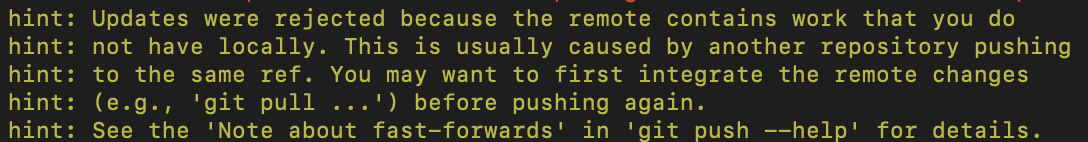
\includegraphics[width=\textwidth]{images/erreur_push_git.png}
    \caption{Message d'erreur quand des modifications ont été faites sur le dépôt git mais pas dans la version locale sur votre ordinateur.}\label{fig:erreur_push_git}
\end{figure}

En effet, après avoir clôner le dépôt, nous avons fait des modifications directement sur GitHub. Puis, nous avons modifié la version locale. Les deux versions n'étant pas identique, il est nécessaire de se mettre-à-jour avant de soumettre nos modifications.

\begin{myexampleblock}{Exercice : Gérer manuellement la fusion}
    \begin{enumerate}
        \item Tapez \texttt{git pull}.
        \item Si vous obtenez une erreur similaire à la figure~\ref{fig:erreur_pull_git}, suivez les étapes suivantes :
        \begin{enumerate}
            \item Tapez \texttt{git config pull.rebase false}.
            \item Tapez \texttt{git pull}.
        \end{enumerate}
        \item Tapez \texttt{git status}.
    \end{enumerate}
\end{myexampleblock}

\begin{myblock}{\href{https://git-scm.com/docs/git-status}{Git status}}
    La commande \code{git status} permet d'afficher l'état du dépôt.
\end{myblock}

\begin{figure}[!h]
    \centering
    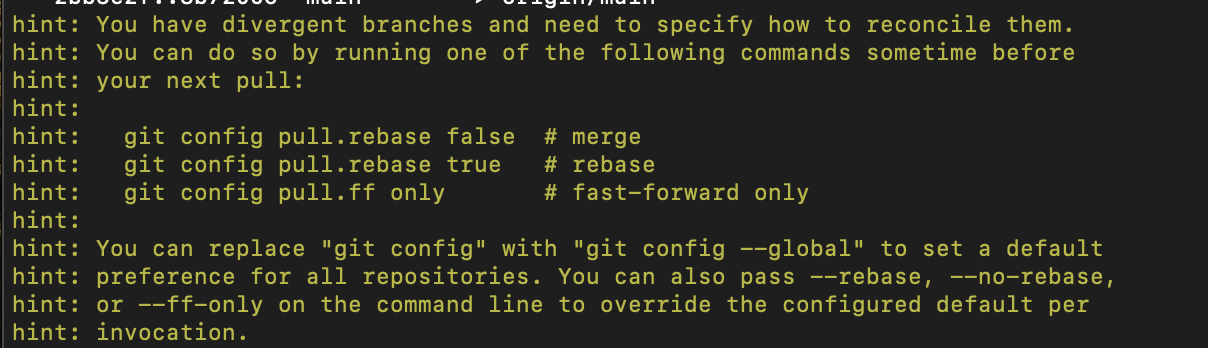
\includegraphics[width=\textwidth]{images/erreur_pull_git.png}
    \caption{Message d'erreur quand des modifications ont été faites sur le dépôt git mais pas dans la version locale sur votre ordinateur.}\label{fig:erreur_pull_git}
\end{figure}

Après toutes ces étapes, vous devriez avoir une sortie similaire à celle de la figure~\ref{fig:git_status}

\begin{figure}[!h]
    \centering
    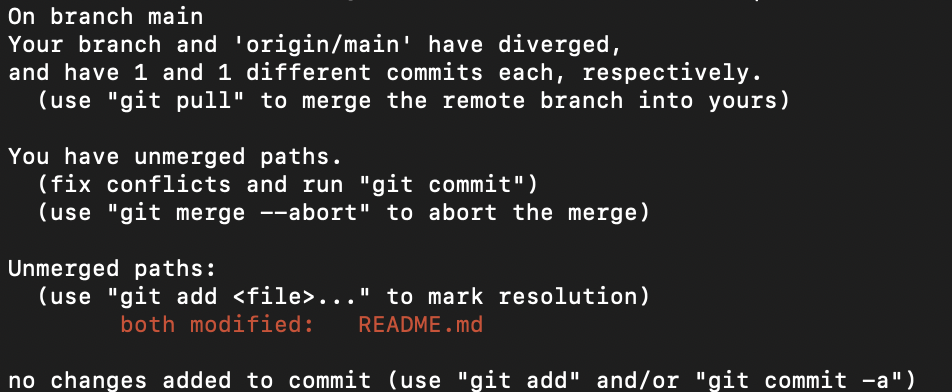
\includegraphics[width=\textwidth]{images/git_status.png}
    \caption{Sortie dans la console après la commande \texttt{git status}.}\label{fig:git_status}
\end{figure}

On voit bien en rouge que les deux branches ont modifiées le README. Nous allons donc ouvrir le README dans votre éditeur de code préféré. Dans le README, vous devriez voir les symboles suivant : \code{<<<<<<<}, \code{=======}, \code{>>>>>>>}, similairement à la figure~\ref{fig:git_merge}.

\begin{figure}[!h]
    \centering
    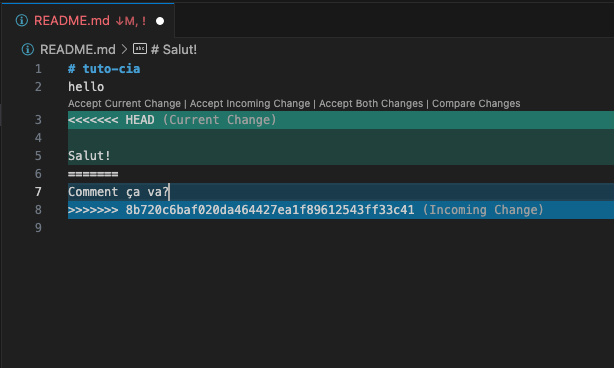
\includegraphics[width=\textwidth]{images/git_merge.png}
    \caption{Apparence du fichier README lorsque la fusion a échoué.}\label{fig:git_merge}
\end{figure}

La section entre \code{<<<<<<<} et \code{=======} correspond au code local en conflit. La section entre \code{=======} et \code{>>>>>>>} correspond au code déjà soumis sur GitHub qui rentre en conflit avec votre code local. Dans la figure~\ref{fig:git_merge}, VSCode propose quatre options pour gérer le conflit. Vous pouvez accepter les modifications locales, accepter les modifications entrantes ou faire un mélange des deux. Si vous savez quelle version choisir, laissez l'éditeur faire son travail et cliquer sur une des deux options. Sinon, vous pouvez manuellement modifier le fichier jusqu'à ce qu'il soit à votre goût. Assurez vous d'enlever les symboles \code{<<<<<<<}, \code{=======}, \code{>>>>>>>}. \\

Suivez maintenant les étapes suivantes pour finaliser la fusion.

\begin{myexampleblock}{Exercice : Finir la fusion}
    \begin{enumerate}
        \item Ouvrez le fichier README dans un éditeur de code.
        \item Faites les modifications nécessaires. Retirez les symboles associés au conflit. 
        \item Dans le terminal, tapez \texttt{git add README.md}.
        \item Tapez \texttt{git commit -m "Mon premier conflit!"}.
        \item Tapez \texttt{git push}.
    \end{enumerate}
\end{myexampleblock}
Normalement, si tout a fonctionné, les modifications devraient apparaître sur GitHub! 

Pour plus d'information sur les conflits, allez voir ici : \href{https://docs.github.com/fr/pull-requests/collaborating-with-pull-requests/addressing-merge-conflicts/resolving-a-merge-conflict-using-the-command-line}{Lien du tutoriel GitHub}.
\section{Fonctionnalités GitHub}
Normalement, avec tout ce qui a été discuté jusqu'à maintenant, vous devriez être en mesure d'utiliser Git et GitHub. Mais, il existe des fonctionnalités de GitHub dont nous n'avons toujours pas parlé. Par exemple, peut-être vous souviendrez-vous avoir vu, lors de la modification du README sur GitHub, l'option \code{Create a new branch for this commit and start a pull request}. Les branches permettent de travailler sans avoir peur de faire une erreur dans le code. De plus, lors d'un travail d'équipe, cela permet à chacun de développer tranquillement sans gérer de fusion, avant de pousser le tout dans la branche principale. 

Un autre outil utile est la création d'\emph{issues} sur GitHub. Les \emph{issues} GitHub permettent de décrire un problème ou une tâche. 

\subsection{Créer des issues}
Tel que mentionné plus haut, les \emph{issues} sont des tickets de tâches qui devront être accomplies plus tard. Ces tickets contiennent un titre et une description, et peuvent être assigner à un membre du dépôt. 

\begin{myexampleblock}{Exercice : Créer un \emph{issue}}
    \begin{enumerate}
        \item Ouvrez votre dépôt GitHub et ouvrez la section \emph{issues}.
        \item Cliquez sur le bouton vert \code{New issue}.
        \item Ajoutez un titre. Je recommande ``Mon premier issue''.
        \item Ajoutez une courte description.
        \item Dans le coin à droite, assignez vous-même à l'issue.
        \item Créez l'issue.
    \end{enumerate}
\end{myexampleblock}
Maintenant que l'\emph{issue} est créé, il sera disponible jusqu'à ce qu'il soit fermé. Dans le cadre de certains gros projets, par exemple \href{https://github.com/scikit-learn/scikit-learn/issues}{Scikit-Learn}, il est possible de reporter un bug ou poser une question. Un \emph{issue} peut être fermé de deux façons différentes : \code{Close as completed} et \code{Close as not planned}. Lorsque vous avez réglé le problème, l'\emph{issue} va être fermée en tant que complétée. Toutefois, si vous ne souhaitez plus réglez le problème, ou c'était une amélioration que vous n'avez pas le temps ou l'envie de faire, vous pouvez fermer l'\emph{issue} en tant que ``non planifié''. 

Après l'ouverture d'une \emph{issue}, GitHub propose automatiquement de créer une branche sur laquelle régler le problème. 

\subsection{Créer une branche}
Nous allons maintenant créer la branche. Sur la branche, vous pouvez faire toutes les modifications en rapport avec le problème que vous résolvez. Lorsque l'\emph{issue} sera réglé, vous pourrez fusionner votre branch avec la branche principale. Créons maintenant la branche. 

\begin{myexampleblock}{Exercice : Créer une branche}
    \begin{enumerate}
        \item Ouvrez l'issue qui vous intéresse.
        \item Cliquez sur \code{Create a branch} en bas à droite.
        \item Modifiez le nom de l'issue pour un nom un peu plus court.
        \item Sélectionnez \code{Checkout locally}.
        \item Cliquez sur le bouton vert \code{Create branch}.
    \end{enumerate}
\end{myexampleblock}

Au lieu de créer la branche sur GitHub, il est aussi possible de l'utiliser avec la commande \code{git branch}. Toutefois, c'est toujours plus facile de passer par GitHub.
\begin{myblock}{\href{https://git-scm.com/docs/git-branch}{git branch}}
    La commande \code{git branch} peut être utilisée pour faire trois choses. 
    \begin{enumerate}
        \item lister les branches : \code{git branch --list}
        \item créer une nouvelle branche nommée \texttt{<nom-de-la-branche>} : \code{git branch <nom-de-la-branche>}
        \item supprimer une branche nommée \texttt{<nom-de-la-branche>}: \code{git branch -d <nom-de-la-branche>}
    \end{enumerate}
\end{myblock}

Pour accéder à la branche, vous pouvez suivre les instructions de GitHub. 
\begin{myexampleblock}{Exercice : Accéder à la branche}
    \begin{enumerate}
        \item Dans le terminal, tapez \code{\texttt{git fetch origin}}.
        \item Entrez \code{\texttt{git checkout <nom-de-la-branche>}}.
    \end{enumerate}
\end{myexampleblock}

\begin{myblock}{\href{https://git-scm.com/docs/git-checkout}{git checkout}}
    La commande \code{git checkout} est généralement utilisée de deux façons différentes.
    \begin{enumerate}
        \item Changer de branche : \code{git checkout <nom-de-la-branche>}
        \item Investiguer un commit : \code{git checkout <numéro-du-commit>}
    \end{enumerate}
\end{myblock}

Modifiez maintenant le README sur la nouvelle branche, puis poussez la modification sur la branche. Nous allons maintenant effectuer une \emph{pull-request}.

\subsection{Pull request}
Les \emph{pull requests} permettent de vérifier les changements qui ont été effectués sur la branche. Elles sont aussi utilisées pour faire vérifier le code par des collègues avant de fusionner les modifications à la branche principale. Vos collègues pourront mettre des commentaires et demander des modifications avant d'accepter la fusion. 

Si vous ne l'avez pas encore fait, faites une modification dans le README sur la nouvelle branche, puis poussez la modification sur la branche. En allant sur GitHub dans la section \code{Pull requests}, vous verrez maintenant un nouveau message disant \code{<nom-de-la-branche> had recent pushes $x$ minutes ago}. Cliquez maintenant sur \code{Compare \& pull request}. 
\begin{myexampleblock}{Exercice : Créer une \emph{pull request}}
    \begin{enumerate}
        \item Cliquez sur \code{Compare \& pull request}.
        \item Ajoutez un titre parlant.
        \item Ajoutez une courte description de la modification.
        \item Cliquez sur le bouton vert \code{Create pull request}.
    \end{enumerate}
\end{myexampleblock}

Normalement, si c'était un projet avec plusieurs coéquipiers, vous seriez amener à ajouter des reviewers. Sans l'approbation des reviewers, vous ne serez pas en mesure de fusionner votre code avec la branche principale. De plus, GitHub vous indique s'il y a un conflit avec la branche principale. Dans ce cas, j'utilise généralement \href{https://gist.github.com/whoisryosuke/36b3b41e738394170b9a7c230665e6b9}{ce tutoriel}.

Après la création d'une \emph{pull request}, vous avez accès à la conversation avec les reviewers, les différents \emph{commit} que vous avez poussé sur la branche ainsi qu'une comparaison entre le code sur la branche principale et les modifications entrantes. 

Quand le code est approuvé, cliquez sur \code{Merge pull request}. Le code sera maintenant fusionné à la branche principale. GitHub vous proposera de 
supprimer la branche. Puisqu'elle ne sera plus utilisée, généralement, vous pouvez la supprimer immédiatement. En fermant la \emph{pull request}, généralement, l'\emph{issue} va être fermée en tant que complétée. 

\subsection{Commandes Git pour quand vous avez fait une erreur}

Assurément, vous allez faire des erreurs en utilisant Git. Ce qui est important, c'est d'être capable de s'en sortir après avoir fait une erreur. Je présente les trois commandes qui me semblent le plus pertinentes.
\begin{myblock}{\href{https://git-scm.com/docs/git-reset}{git reset}}
    La commande \code{git reset <numéro-du-commit>} permet de supprimer les modifications qui ont été faites depuis le \emph{commit} sélectionné. Si vous utilisez le drapeau \code{--soft}, les \emph{commits} sont supprimés mais pas les modifications. Si vous utilisez le drapeau \code{--hard}, les \emph{commits} et les modifications sont supprimées.
\end{myblock}
 
\begin{myblock}{\href{https://git-scm.com/docs/git-revert}{git revert}}
    La commande \code{git revert <numéro-du-commit>} permet d'inverser les modifications faites dans un \emph{commit}. Cette commande crée un nouveau \emph{commit} avec exactement l'inverse des modifications du \emph{commit} choisi. Pour plus d'information, voir ce \href{https://stackoverflow.com/questions/19032296/how-to-use-git-revert}{post de StackOverflow}.
\end{myblock}

\begin{myblock}{git commit --amend}
    La commande \code{git commit} peut être utilisée avec le drapeau \code{--amend} pour faire des modifications aux commits qui n'ont pas encore été poussés. Cette commande permet de faire différents types de modifications, je vous propose donc deux sources différentes pour apprendre à la connaître : \href{https://www.atlassian.com/git/tutorials/rewriting-history}{site de Git} et \href{https://www.atlassian.com/git/tutorials/rewriting-history}{site d'Atlassian.} 
\end{myblock}

Il existe plein d'autres commandes git qui peuvent être utilisées, mais qui sont trop spécialisées et ne sont pas assez utilisées pour qu'elles soient présentées dans ce tutoriel. Je vous recommande la \href{https://git-scm.com/docs}{documentation de Git} pour toutes vos questions, ainsi que StackOverflow. Je vous recommande de plus la \href{https://training.github.com/downloads/fr/github-git-cheat-sheet.pdf}{cheat sheet de GitHub}!

\end{document}